% Figure for the flipbook of strategies over time

\begin{figure}
\center

	\begin{subfigure}[t]{0.3\textwidth}
	\centering
	
\includegraphics[width=\stratgraphwidth]{images/findings/round1/flipbook_a.png}
	\caption{Starting Weights}
	\end{subfigure}
	~
	\begin{subfigure}[t]{0.3\textwidth}
	\centering
	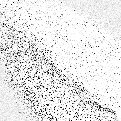
\includegraphics[width=\stratgraphwidth]{images/findings/round1/flipbook_b.png}
	\caption{After 200,000 games played}
	\end{subfigure}
	~
	\begin{subfigure}[t]{0.3\textwidth}
	\centering
	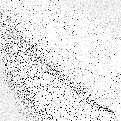
\includegraphics[width=\stratgraphwidth]{images/findings/round1/flipbook_c.png}
	\caption{After 400,000 games played}
	\end{subfigure}

	\begin{subfigure}[t]{0.3\textwidth}
	\centering
	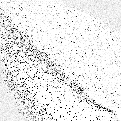
\includegraphics[width=\stratgraphwidth]{images/findings/round1/flipbook_d.png}
	\caption{After 600,000 games played}
	\end{subfigure}
	~
	\begin{subfigure}[t]{0.3\textwidth}
	\centering
	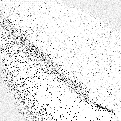
\includegraphics[width=\stratgraphwidth]{images/findings/round1/flipbook_e.png}
	\caption{After 800,000 games played}
	\end{subfigure}
	~
	\begin{subfigure}[t]{0.3\textwidth}
	\centering
	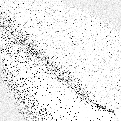
\includegraphics[width=\stratgraphwidth]{images/findings/round1/flipbook_f.png}
	\caption{Final Weights}
	\end{subfigure}

\caption{%
	Training weights representation for an agent's \handmaxavg\
	strategy when that agent is the pone
	over the course of the one million games of Round 1.
	In these images, the y-axis represents the player's own score,
	the x-axis the opponent's score,
	with the origin starting at the top-left of the image.
	% N.B. This is correct of generated images from the python code
	%	as of 2018-03-08 19:12.
	% no later modifications will be made from the python code directly to
	% save myself the headache. maybe this will be converted later to be
	% more easily human understood
	% Rotate 90 deg counter-clockwise will make x=my_score, y=opp_score
}
\label{fig_r1-flip}
\end{figure}
